\documentclass{article}

\usepackage[utf8]{inputenc}
\usepackage{longtable}
\usepackage{authblk}
\usepackage{adjustbox}
\usepackage{natbib}

\title{Indice de Desarrollo Humano en Colombia}
% autores
\renewcommand\Authand{, y }
\author[1]{\normalsize Camilo Andrés Nieto}
\author[2]{\normalsize Angela María Romero}

\affil[1,2]{\small  Facultad de Ingeniería, Universidad de los Andes\\
Bogotá, Colombia
\texttt{{ca.nieto11,am.romero14}@uniandes.edu.co}}

\usepackage{Sweave}
\begin{document}
\Sconcordance{concordance:ProyectoFinal.tex:ProyectoFinal.Rnw:%
1 18 1 1 0 18 1 1 8 1 5 1 12 15 0 1 2 2 1 1 21 1 5 5 1 1 17 1 5 7 1 1 %
13 12 0 1 10 13 0 1 3 3 1 1 4 1 2 6 1 1 10 31 0 1 6 5 1 1 75 2 1 1 17 1 %
2 8 1}


\maketitle

\renewcommand{\tablename}{Tabla}
\renewcommand{\figurename}{Figura}

\begin{abstract}
Este es mi primer trabajo en exploracion y modelamiento de indices usando LATEX. Este trabajo lo he hecho bajo la filosofía de trabajo replicable.
\end{abstract}

\section*{Introducción}

Aqui les presento mi investigacion sobre el indice IDH en Colombia. Los indices los conseguí de wikipedia, espero que les gusten mucho.

\section{Exploración Univariada}\label{univariada}

En esta sección exploro cada índice.


% Table created by stargazer v.5.2.2 by Marek Hlavac, Harvard University. E-mail: hlavac at fas.harvard.edu
% Date and time: vie., jun. 29, 2018 - 6:43:37 p. m.
\begin{table}[!htbp] \centering 
  \caption{Medidas estadísticas} 
  \label{stats} 
\begin{tabular}{@{\extracolsep{5pt}}lccccc} 
\\[-1.8ex]\hline 
\hline \\[-1.8ex] 
Statistic & \multicolumn{1}{c}{Mean} & \multicolumn{1}{c}{St. Dev.} & \multicolumn{1}{c}{Max} & \multicolumn{1}{c}{Min} & \multicolumn{1}{c}{Median} \\ 
\hline \\[-1.8ex] 
IDH & 0.802 & 0.042 & 0.879 & 0.691 & 0.804 \\ 
Población.Cabecera & 1,196,730.000 & 1,982,287.000 & 10,070,801 & 13,090 & 717,197 \\ 
Población.Resto & 360,590.300 & 331,887.600 & 1,428,858 & 21,926 & 268,111.5 \\ 
Población.Total & 1,557,320.000 & 2,202,522.000 & 10,985,285 & 43,446 & 1,028,429 \\ 
\hline \\[-1.8ex] 
\end{tabular} 
\end{table} 
\begin{figure}[h]
\centering
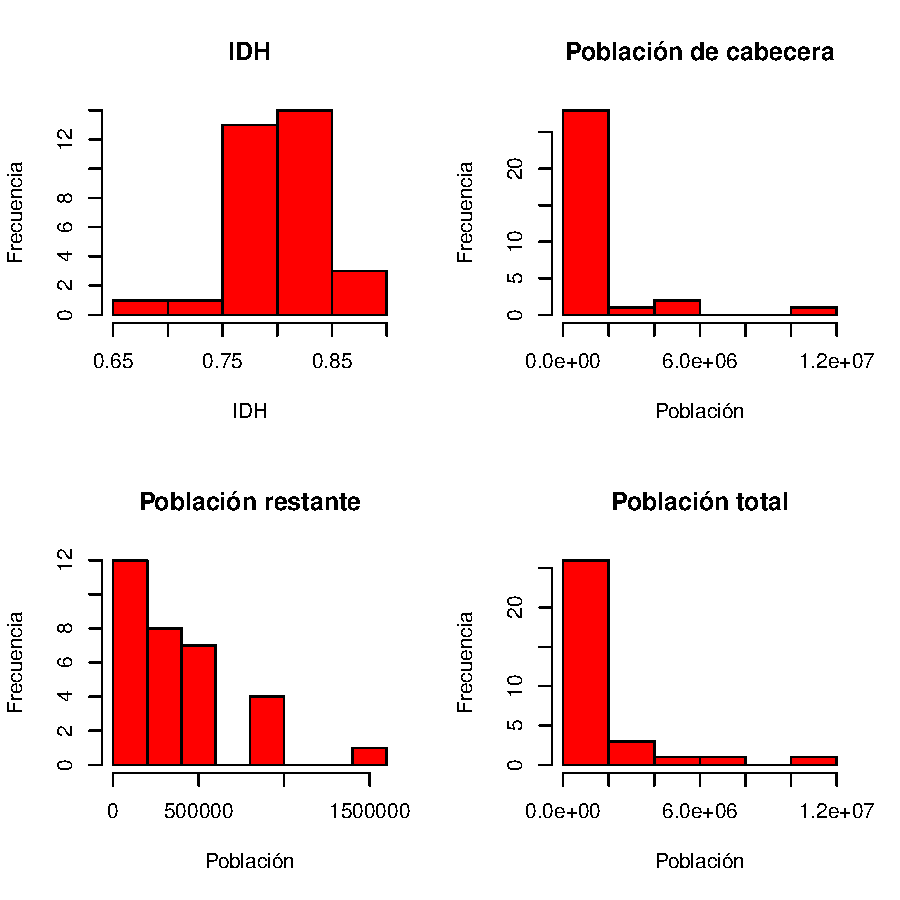
\includegraphics{ProyectoFinal-expUnivariadaGraficos}
\caption{Histogramas de los datos}
\label{histogramas}
\end{figure}

\begin{figure}[h]
\centering
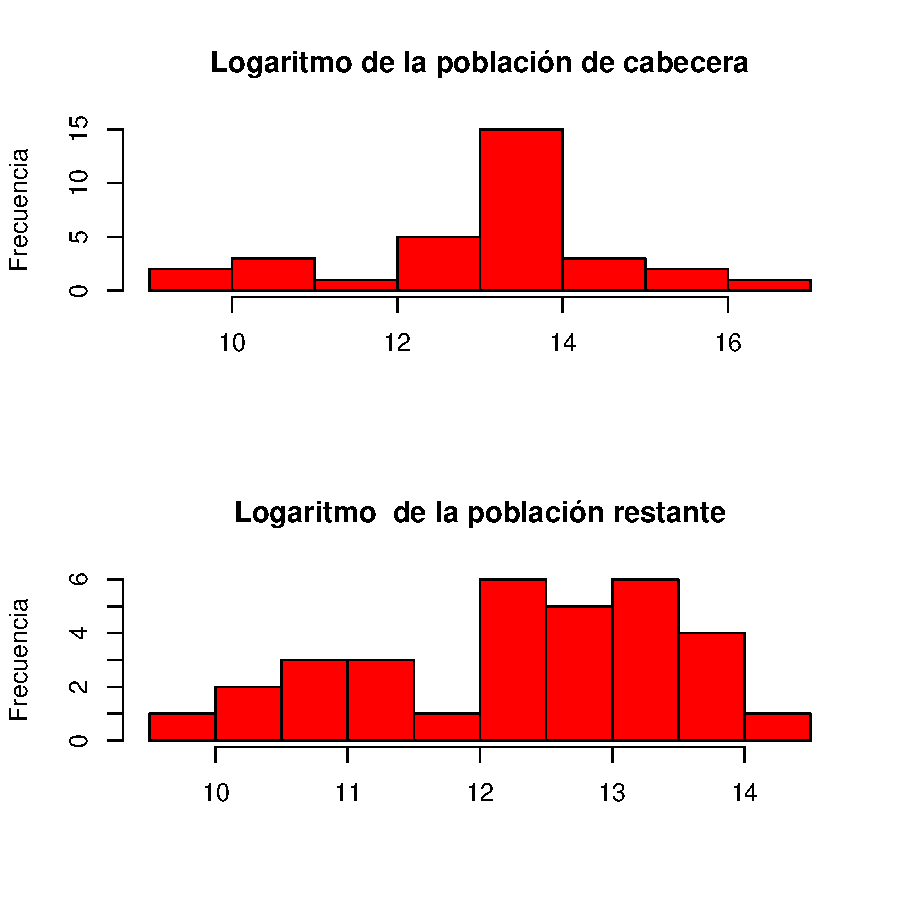
\includegraphics{ProyectoFinal-graficosSesgo}
\caption{Histogramas de los logaritmos}
\label{histogramasLog}
\end{figure}

\clearpage

\section{Exploración Bivariada}

% Table created by stargazer v.5.2.2 by Marek Hlavac, Harvard University. E-mail: hlavac at fas.harvard.edu
% Date and time: vie., jun. 29, 2018 - 6:43:37 p. m.
\begin{table}[!htbp] \centering 
  \caption{Impacto de la poblacion en el el IDH} 
  \label{} 
\begin{tabular}{@{\extracolsep{5pt}} cc} 
\\[-1.8ex]\hline 
\hline \\[-1.8ex] 
cabeLog & restoLog \\ 
\hline \\[-1.8ex] 
$0.487$ & $0.177$ \\ 
\hline \\[-1.8ex] 
\end{tabular} 
\end{table} % Table created by stargazer v.5.2.2 by Marek Hlavac, Harvard University. E-mail: hlavac at fas.harvard.edu
% Date and time: vie., jun. 29, 2018 - 6:43:37 p. m.
\begin{table}[!htbp] \centering 
  \caption{Correlación entre las variables independientes} 
  \label{} 
\begin{tabular}{@{\extracolsep{5pt}} ccc} 
\\[-1.8ex]\hline 
\hline \\[-1.8ex] 
 & cabeLog & restoLog \\ 
\hline \\[-1.8ex] 
cabeLog & 1 &  \\ 
restoLog & 0.84 & 1 \\ 
\hline \\[-1.8ex] 
\end{tabular} 
\end{table} 
\begin{figure}[h]
\centering 
\begin{adjustbox}{width=8cm,height=7cm,clip,trim=0cm 0cm 0cm 0cm}
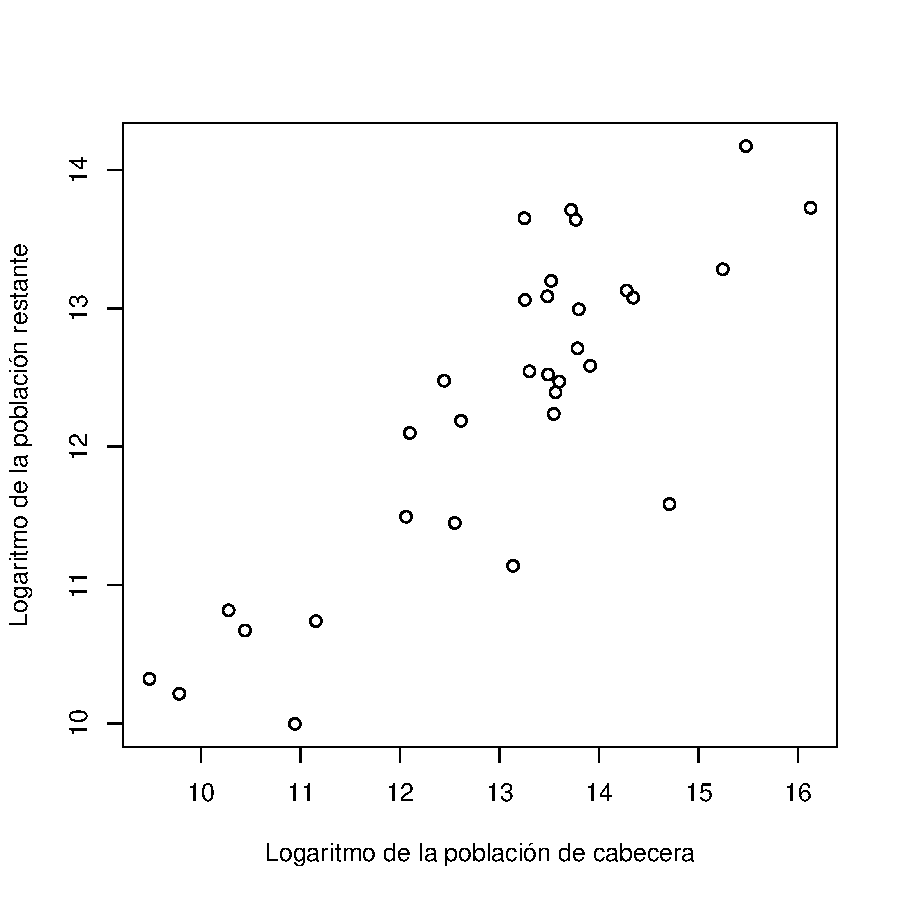
\includegraphics{ProyectoFinal-CorrPlotExpBivariada}
\end{adjustbox}
\caption{Gráfica de corrlación entre los logaritmos de las poblaciones}
\label{corrPlot}
\end{figure}

\clearpage
\section{Modelos de regresión}
% Table created by stargazer v.5.2.2 by Marek Hlavac, Harvard University. E-mail: hlavac at fas.harvard.edu
% Date and time: vie., jun. 29, 2018 - 6:43:37 p. m.
\begin{table}[!htbp] \centering 
  \caption{Modelos de Regresión} 
  \label{regresiones} 
\begin{tabular}{@{\extracolsep{5pt}}lcc} 
\\[-1.8ex]\hline 
\hline \\[-1.8ex] 
 & \multicolumn{2}{c}{\textit{Dependent variable:}} \\ 
\cline{2-3} 
\\[-1.8ex] & \multicolumn{2}{c}{IDH} \\ 
\\[-1.8ex] & (1) & (2)\\ 
\hline \\[-1.8ex] 
 cabeLog & 0.013$^{***}$ & 0.031$^{***}$ \\ 
  & (0.004) & (0.007) \\ 
  & & \\ 
 restoLog &  & $-$0.030$^{***}$ \\ 
  &  & (0.010) \\ 
  & & \\ 
 Constant & 0.634$^{***}$ & 0.766$^{***}$ \\ 
  & (0.055) & (0.065) \\ 
  & & \\ 
\hline \\[-1.8ex] 
Observations & 32 & 32 \\ 
R$^{2}$ & 0.238 & 0.425 \\ 
Adjusted R$^{2}$ & 0.212 & 0.385 \\ 
Residual Std. Error & 0.037 (df = 30) & 0.033 (df = 29) \\ 
F Statistic & 9.347$^{***}$ (df = 1; 30) & 10.706$^{***}$ (df = 2; 29) \\ 
\hline 
\hline \\[-1.8ex] 
\textit{Note:}  & \multicolumn{2}{r}{$^{*}$p$<$0.1; $^{**}$p$<$0.05; $^{***}$p$<$0.01} \\ 
\end{tabular} 
\end{table} 
\clearpage

\section{Exploración Espacial}

Se utilizan técnicas de k-means propuesta por MacQueen \cite{macqueen_methods_nodate} para identificar conglomerados de regiones

\begin{figure}[h]
\centering
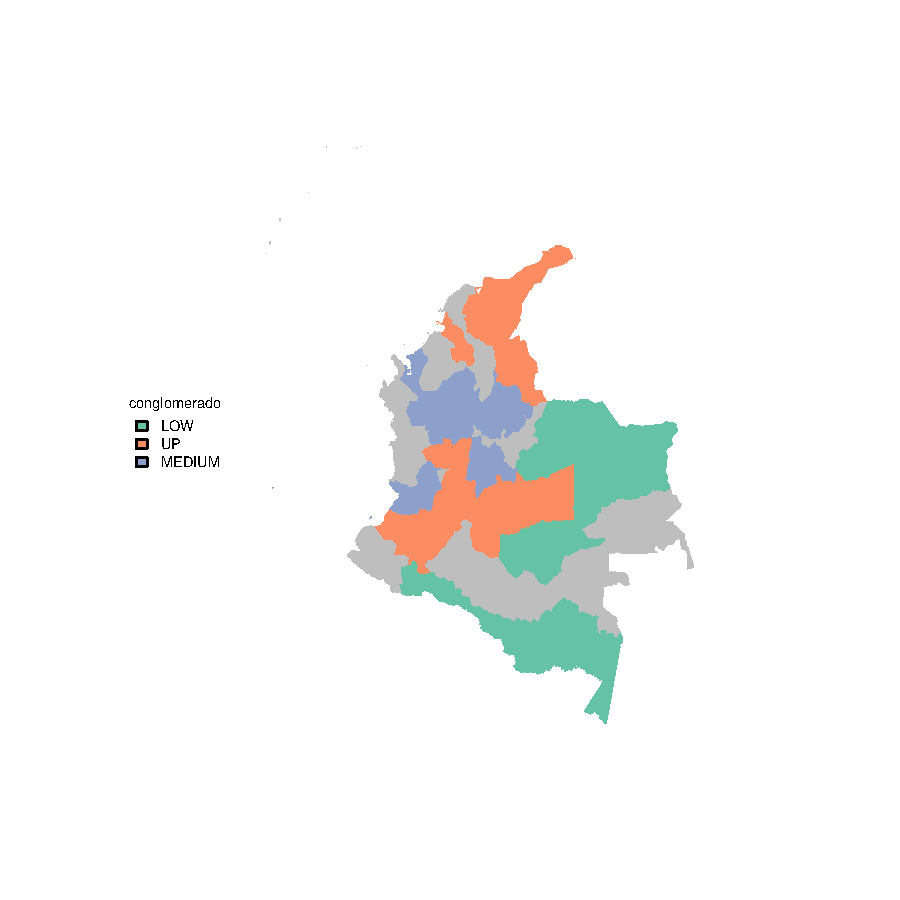
\includegraphics{ProyectoFinal-MapPaint}
\caption{Mapa del IDH}
\label{map}
\end{figure}

\bibliographystyle{abbrv}
\renewcommand{\refname}{Bibliografía}
\bibliography{Proyecto}

\end{document}
